%!TEX TX-program = xelatex
%
%%%%%%%%%%%%%%%%%%%%
%
% Title: 11 220518 向量与复数
% Author: Eason S.
% Date: 220518
% Institude: Shanghai Experimental School
% Email: eason.syc@icloud.com
% GitHub: https://github.com/EasonSYC
% GitHub Repository: https://github.com/EasonSYC/Maths_Error
%
%%%%%%%%%%%%%%%%%%%%

\documentclass[8pt]{article}
\usepackage{allan-eason}

\usetikzlibrary{positioning}
\usetikzlibrary{svg.path}

\graphicspath{ {./images/} }

\newcommand{\Date}{220518}
\newcommand{\Test}{向量与复数}

\newcommand{\Author}{Eason S.}
\newcommand{\Title}{\textcolor{allandarkblue}{\Date}\ \textcolor{allancyan}{\Test}\ 题目选解}

\author{\Author}
\title{\Title}
\date{}

\geometry{a4paper, scale=0.8}

\lhead{\Title}

\begin{document}

	\maketitle

	\tableofcontents

	\section{复数}
		\calword{虚数的定义:} 虚数可看作\defword{实数与虚数单位\(i\)}的乘积, 其中规定\(i^2 = -1\). 因此, \(0\)可同时视为虚数和实数.

		\calword{虚数单位:} 虚数单位一般排版为\(i\)或\(\mathrm{i}\), 本作者的系列作品将以前者\(i\)进行排版. 若遇到有\(i\)作为变量的情景, 会选用\(j\)对虚数单位进行代替, 但会补充说明.
		
		\calword{虚数和负数算数平方根:} 我们可以说\(i = \sqrt{-1}, -i = -\sqrt{-1}\), 但是\(i = -\sqrt{-1}, -i = \sqrt{-1}\)的对应也未尝不可. 换而言之, \defword{对于负数的开根号对应的虚数并没有自然的定义}. \cite{wiki-img}

		\calword{虚数的性质:} 可以在虚数用\(ki\)中的\(k\)定义序, 但是虚数上定义的序和复数的运算是不相容的. 即, 虚部和实部均不为\(0\)的数\defword{不可进行简单的大小比较} (无法定义与加法和乘法相融的序). \cite{wiki-img}

		\calword{虚数集的表示:} 虚数集\defword{没有公认的单字母表达方式}, 可选的有\(i\RR, \II, \im, \Im\), 本作者的系列作品将以\(\II\)的方式进行排版.

		\calword{复数的定义:} 复数为实数的延伸, \defword{可以一般的表达为} \(z = a + bi, a, b \in \RR\).
		
		\calword{复数的虚部与实部:} 我们定义\(z\)的\defword{实部}为\(\Re (z) = \re z = a\), \defword{虚部}为\(\Im (z) = \im z = b\). 本作者的系列作品将以前者排版.
		
		\calword{复数集的表示:} 记复数集 (域) 为\(\CC\).

		\calword{复数域上的序:} 简而言之, 在\(\CC\)上\defword{不可建立与其加法和乘法相融的全序关系}, 即不存在全序\(\preceq\), 使得\(\forall z_1, z_2 \in \CC: 0 \preceq z_1, z_2 \Rightarrow 0 \preceq z_1, z_2, 0 \preceq z_1, z_2\). \cite{wiki-comp}

		\calword{复平面:} 绘制笛卡尔坐标系, 横轴称之为\defword{实数轴}, 纵轴称之为\defword{虚数轴}, 则该平面上的点与\(\CC\)中的元素\defword{一一对应}.

		\calword{复数与极坐标:} 定义复数的\defword{模长/绝对值}为\(r = \abs{z} = \sqrt{a^2 + b^2} > 0\), 辐角\(\varphi = \arg z \in \left(-\pi, \pi\right]\), 有\(x = r \cos \varphi, y = r \sin \varphi\). 此即为\defword{极坐标}.

		\calword{复数的三角形式:} 有\(z = r \left(\cos \varphi + i \sin \varphi\right)\), 此即为\defword{三角形式}.

		\calword{复数的指数形式:} 由\defword{欧拉公式}\(e^{ix} = \cos x + i \sin x\), 有\(z = r e^{i\varphi}\), 此即为\defword{指数形式}. \cite{wiki-comp}

		\calword{共轭复数:} 复数\(z = a + bi\)的\defword{共轭复数}\(\overline{z} = a - bi\), \(z = re^{i \theta} \Rightarrow \overline{z} = re^{-i\theta}\). 显然有对于复数\(z\)与\(w\)有\(\overline{z + w} = \overline{z} + \overline{w}, \overline{zw} = \overline{z} \cdot \overline{w}\). 同时有\defword{在复数域上的函数\(\phi\)若能表达成实系数幂级数}, 有\(\phi(z) = \overline \phi(z)\). \cite{wiki-comconj}
		
		\calword{复数的距离:} 定义复数\(z, w\)的\defword{距离}为\(d(z, w) = \abs{z - w} = \abs{w - z}\). 这使复数域变为了\defword{度量空间}, 我们亦可以谈极限和连续. 加法, 乘法和除法都是连续的运算. \cite{wiki-comp} \cite{wiki-metric}

		\calword{实数的复指数幂:} 定义\defword{实数的复指数幂} \(a^z = e^{z \cdot \ln a}\).

		\calword{复数与矩阵:} 复数可看作\defword{旋转及缩放二维位置矢量的\(2 \times 2\)实矩阵}, 即
		
		\begin{displaymath}		
			a + bi \leftrightarrow \left[
				\begin{array}{cc}
					a & -b\\
					b & a
				\end{array}
			\right] = r \left[
				\begin{array}{cc}
					\cos \varphi & - \sin \varphi\\
					\sin \varphi & \cos \varphi
				\end{array}
			\right] = r \exp \left( \varphi \left[
				\begin{array}{cc}
					0 & -1\\
					1 & 0
				\end{array}
			\right] \right).
		\end{displaymath}

		复数的绝对值即为对应矩阵\(\mathbf{Z}\)的行列式的值的平方根\(\displaystyle \sqrt{\det \mathbf{Z}}\).

		\calword{代数学基本定理, 复数域的代数封闭性:} 满足\(p(z) = 0\)的复数\(z\)是多项式\(p\)的\defword{根}, 而\defword{代数学基本定理}指出, 所有\(n\)次多项式, 无论实数或复数系数, 都恰好有\(n\)个复数根. 该定理等价于\defword{复数域是代数闭域}.

		\calword{通过环与理想定义复数域:} 复数域是实数域的\defword{代数闭包}, 是\defword{多项式环}\(\RR[X]\)经由\defword{理想}\(\ang{X^2 + 1}\)显生出的\defword{商环}: \cite{wiki-comp}

		\begin{displaymath}
			\CC = \RR[X] / \left(X^2 + 1\right).
		\end{displaymath}

		多项式\(X^2 + 1\)是一个\defword{不可约多项式}, 使得复数环是一\defword{域}, \(X\)在商环内对应着虚数单位\(i\).

	\section{填空题}
		\begin{easonproblem}
			已知三点\(A(2, 3), B(4, 3), C\displaystyle\left(5. \frac{m}{2}\right)\)在同一直线上, 则\(m\)的值为?.
			\subproblem
			\answord{\(12\).} 直线的方程.
		\end{easonproblem}
		
		\begin{easonproblem}
			设\(\vec{e}_1\)与\(\vec{e}_2\)是两个不共线的向量, 已知\(\ray{AB} = 2 \vec{e}_1 + k \vec{e}_2, \ray{CB} = \vec{e}_1 + 3\vec{e}_2, \ray{CD} = 2\vec{e}_1 - \vec{e}_2\), 则当\(A, B, C\)三点共线时, \(k\)的值为?.
			\subproblem
			\answord{\(-8\).} 向量的平行.
		\end{easonproblem}

		\begin{easonproblem}
			已知\(z \in \II, \displaystyle \frac{z+2}{1-i} \in \RR\), 则\(z\)的值为?.
			\subproblem
			\answord{\(-2i\).} 复数的运算.
		\end{easonproblem}

		\begin{easonproblem}
			计算:
			\begin{displaymath}
				\left\{ \left[
						i^100 - \left(
							\frac{1-i}{1+i}
						\right)^5
					\right] + \left(
						\frac{1+i}{\sqrt{2}}^2
					\right)
				\right\}(1+2i).
			\end{displaymath}
			\subproblem
			\answord{\(-3+4i\).} 复数的运算.
		\end{easonproblem}
		
		\begin{easonproblem}
			在复数范围内分解因式:
			\begin{displaymath}
				x^6 + 2x^4 - x^2 - 2.
			\end{displaymath}
			\subproblem
			\answord{\((x+1)(x-1)(x-\sqrt{2}i)(x+\sqrt{2}i)(x-i)(x+i)\).} 复数下的因式分解, 实系数方程的复根.
		\end{easonproblem}

		\begin{easonproblem}
			已知关于\(x\)的方程\(x^2 - (2i - 1)x + m - i = 0\)有实根, 则实数\(m\)的值为?.
			\subproblem
			\answord{\(\displaystyle \frac{1}{4}\).} 实数运算的封闭性.
		\end{easonproblem}

		\begin{easonproblem}
			已知\(z_1, z_2 \in \CC, x \in \RR\), 以下四个关系式中能够成立的有?.
			\begin{multicols}{2}
				\begin{enumerate}[label = \calword{(\arabic*)}]
					\item \(\abs{z_1} \leq 1 \Leftrightarrow -1 \leq z_1 \leq 1\);
     				\item \(\abs{x} \leq 1 \Leftrightarrow -1 \leq x \leq 1\);
         			\item \(\abs{z_1} + \abs{z_2} = 0 \Leftrightarrow z_1 = z_2 = 0\);
            		\item \(\abs{z_1} = \abs{z_2} \Leftrightarrow z_1 = \pm z_2\). 
				\end{enumerate}				
			\end{multicols}
			\subproblem
			\answord{\calword{(2)(3)}.} 复数的模.
		\end{easonproblem}

		\begin{easonproblem}
			设\(z \in \CC\)满足\(\displaystyle \frac{1-z}{1+z} = i\), 则\(\abs{1+z}\)的值为?.
			\subproblem
			\answord{\(\sqrt{2}\).} 复数的运算, 复数的模.
		\end{easonproblem}

		\begin{easonproblem}
			如图, 在\(\triangle ABC\)中, \(\angle BAC = 90\degree, AB = 6, D\)在斜边\(BC\)上, \(CD = 2DB\), 则\(\ray{AB} \cdot \ray{CD}\)的值为?.
			\begin{center}		
				\begin{tikzpicture}
					\draw[black] (0, 0)--(6, 0)--(4, 1)--(0, 3)--(0, 0)--(4, 1) node at (0, 0) [anchor = north east] {\(A\)} node at (6, 0) [anchor = north west] {\(B\)} node at (0, 3) [anchor = south east] {\(C\)} node at (4, 1) [anchor = south west] {\(D\)};
				\end{tikzpicture}
			\end{center}
			\subproblem
			\answord{\(27\).} 向量的运算.
			\begin{align}
				\ray{AB} \cdot \ray{CD} &= \ray{AB} \cdot \left(\frac{2}{3} \ray {CB}\right)\\
				                        &= \frac{2}{3} \ray{AB} \cdot \ray{CB}\\
										&= \frac{2}{3} \ray{AB} \cdot \left(\ray{CA} + \ray{AB}\right)\\
										&= \frac{2}{3} \left(\ray{AB} \cdot \ray{CA} + \ray{AB} \cdot \ray{AB}\right)\\
										&= \frac{2}{3} \left(0 + 36\right) \left(\text{注意到}AC \perp BC, \ray{AB}^2 = AB^2 = 6^2 = 36\right)\\ 
										&= \frac{2}{3} \times 36\\
										&= 24.
			\end{align}
		\end{easonproblem}

		\begin{easonproblem}
			如图所示: \(\triangle{ABC}\)中, 点\(O\)是\(BC\)中点. 过点\(O\)的直线分别交直线\(AB, AC\)于不同两点\(M, N\). 若\(\ray{AB} = m\ray{AM}, \ray{AC} = n\ray{AN}\), 则\(m+n\)的值为?.
			\begin{center}
				\begin{tikzpicture}
					\draw[black] (0, 0)--(3, 0)--(2, 2)--(0, 0) node at (0, 0) [anchor = east] {\(B\)} node at (3, 0) [anchor = west] {\(C\)} node at (2, 2) [anchor = south] {\(A\)};
					\draw[black] (0, 0)--(-1.5, -1.5)--(2.75, 1) node at (-1.5, -1.5) [anchor = north] {\(M\)} node at (1.5, 0) [anchor = north west] {\(O\)} node at (2.5, 1) [anchor = south] {\(N\)};
				\end{tikzpicture}
			\end{center}
			\subproblem
			\answord{\(2\).} Menelaus定理.

			由Menelaus定理显然有
			\begin{displaymath}
				\frac{AM}{MB} \cdot \frac{BO}{OC} \cdot \frac{CN}{NA} = 1,
			\end{displaymath}
			代入\(\ray{AB} = m\ray{AM}, \ray{AC} = n\ray{AN}, BO = OC\)有
			\begin{displaymath}
				\frac{1}{1 - m} \cdot \frac{n - 1}{1} = 1,
			\end{displaymath}
			即
			\begin{displaymath}
				m + n = 2
			\end{displaymath}
		\end{easonproblem}

		\begin{easonbigproblem}
			设\(\vec{a}, \vec{b}, \vec{c}\)是平面内互不平行的三个向量, \(x \in \RR\), 有下列命题:
			\begin{enumerate}[label=\calword{(\arabic*)}]
				\item 方程\(\vec{a} x^2 + \vec{b} x + \vec{c} = \vec{0} (a \neq \vec{0})\)不可能有两个不同的实数解;
				\item 方程\(\vec{a} x^2 + \vec{b} x + \vec{c} = \vec{0} (a \neq \vec{0})\)有实数解的充要条件是\(\vec{b}^2 - 4 \vec{a} \cdot \vec{c} \geq 0\);
				\item 方程\(\vec{a}^2 x^2 + 2\vec{a} \cdot \vec{b} x + \vec{b}^2 = 0\)有唯一的实数解\(x = - \displaystyle \frac{\vec{b}}{\vec{a}}\);
				\item 方程\(\vec{a}^2 x^2 + 2\vec{a} \cdot \vec{b} x + \vec{b}^2 = 0\)没有实数解.
			\end{enumerate}
			\subbigproblem
			\answord{\calword{(1)(4)}.} 向量的运算, 一元二次方程.
			\begin{enumerate}[label=\calword{(\arabic*)}]
				\item 对方程\(\vec{a} x^2 + \vec{b} x + \vec{c} = \vec{0} (a \neq \vec{0})\)进行变形, 有
					\begin{displaymath}
						\vec{c} = -x^2 \vec{a} - x\vec{b},
					\end{displaymath}
					由平面向量分析基本定理可得, 该方程至多一解.
				\item 该方程是向量的方程, 不能按实系数一元二次方程的判别式进行判断 (此处不作证明).
				\item 该方程为实系数一元二次方程, 有判别式
					\begin{displaymath}
						\Delta = 4 \vec{a} \cdot \vec{b}^2 - 4 \vec{a}^2 \cdot \vec{b}^2 < 0,
					\end{displaymath}
					则方程没有实数解.
				\item 正确.
			\end{enumerate}
		\end{easonbigproblem}

		\begin{easonbigproblem}
			如图, \(OM \parallel AB\), 点\(P\)在由射线\(OM\), 线段\(
				OB\)及\(AB\)的延长线围成的区域内 (不含边界) 运动, 且\(\ray{OP} = x \ray{OA} + y \ray{OB}\), 则\(x\)的取值范围是?; 当\(x = -\displaystyle\frac{1}{2}\)时, \(y\)的取值范围是?.
			\begin{center}
				\begin{tikzpicture}[scale = 0.5]
					\draw[black, ->] (0, 0)--(6, 0)--(5, 3) node at (0, 0) [anchor = north east] {\(O\)} node at (6, 0) [anchor = north west] {\(A\)} node at (5, 3) [anchor = south west] {\(B\)};
					\draw[black, ->] (0, 0)--(-1, 3) node at (-1, 3) [anchor = west] {\(M\)};
					\draw[black, ->] (0, 0)--(5, 3);
					\draw[black, ->] (0, 0)--(3, 4) node at (3, 4) [anchor = south] {\(P\)};
					\draw[black, dashed] (-1, 3)--(-3, 9);
					\draw[black, dashed] (5, 3)--(3, 9);
				\end{tikzpicture}
			\end{center}
			\subbigproblem
			\answord{\(\displaystyle (-\infty, 0); \left(\frac{1}{2}, \frac{3}{2}\right)\).} 向量的运算.

			由向量加法的平行四边形法则, \(OP\)为平行四边形的对角线, 该四边形是以\(OB\)和\(OA\)的反向延长线为两邻边, 故\(x\in (-\infty, 0)\).

			当\(x = -\displaystyle \frac{1}{2}\)时, 要使\(P\)点落在指定区域内, 作\(\ray{OC} = - \displaystyle \frac{1}{2} \ray{OA}\), 作共线三点的\(ODC\)所在直线\(\parallel OB\), 交\(OM\)于\(D\), 交\(AB\)于\(E\).
			
			显然有\(CD = \displaystyle \frac{1}{2} OB, CE = \frac{3}{2} OB\), 则\(y \in \displaystyle \left(\frac{1}{2}, \frac{3}{2}\right)\).
		\end{easonbigproblem}

	\section{解答题}
		\begin{easonproblem}
			已知复数\(z_1\)满足\((z_1 - 2)(1 + i) = 1 - i\), 复数\(z_2\)有\(\Im z_2 = 2\), 且\(z_1 \cdot z_2 \in \RR\), 求\(z_2\).
			\subproblem
			\answord{\(z_2 = 4 + 2i\).} 复数的运算.
		\end{easonproblem}

		\begin{easonproblem}
			已知\(\abs{\vec{a}} = \sqrt{2}, \abs{\vec{b}}=2, \ang{\vec{a}, \vec{b}} = 45\degree\), 求使向量\(\vec{a} + \lambda \vec{b}\)与\(\lambda \vec{a} + \vec{b}\)的夹角是锐角时的\(\lambda\)的取值范围.
			\subproblem
			\answord{\(\displaystyle \lambda \in \left(- \infty, \frac{-3 - \sqrt{5}}{2}\right) \cup \left(\frac{-3 - \sqrt{5}}{2}, 1\right) \cup \left(1, +\infty\right)\).} 向量的位置关系.

			不妨设\(\vec{a} = (1, 1), \vec{b} = (2, 0)\), 则有\(\vec{a} + \lambda \vec{b} = (2\lambda + 1, 1), \lambda \vec{a} + \vec{b} = (\lambda + 2, \lambda)\), 于是有\(\left(\vec{a} + \lambda \vec{b}\right)\left(\lambda \vec{a} + \vec{b}\right) = 2 \lambda^2 + 6\lambda + 2,\) 于是有
			\begin{displaymath}
				\left\{
					\begin{array}{rcl}
						2\lambda^2 + 6 \lambda + 2 &>& 0\\
						2\lambda + 1 &\neq& \frac{\lambda+2}{\lambda}
					\end{array}
				\right.
			\end{displaymath}
			即可解出答案.
		\end{easonproblem}

		\begin{easonbigproblem}
			已知\(\vec{a}, \vec{b}\)是两个不共线的非零向量,
			\begin{enumerate}[label = \calword{(\arabic*)}]
				\item 设\(\ray{OA} = \vec{a}, \ray{OB} = t \vec{b}, t \in \RR, \ray{OC} = \displaystyle \frac{1}{3} \left(\vec{a} + \vec{b}\right)\), 当\(A, B, C\)三点共线时, 求\(t\)的值.
    			\item 如图, 若\(\vec{a} = \ray{OD}, \vec{b} = \ray{OE}, \ang{\vec{a}, \vec{b}} = 120\degree, \abs{\vec{a}} = \abs{\vec{b}} = 1,\) 点\(P\)是以\(O\)为圆心的圆弧\(\arc{DE}\)上一动点, 设\(\ray{OP} = x \ray{OD} + y \ray{OE}, x, y \in \RR\), 求\(x + y\)的最大值.
				\begin{center}
					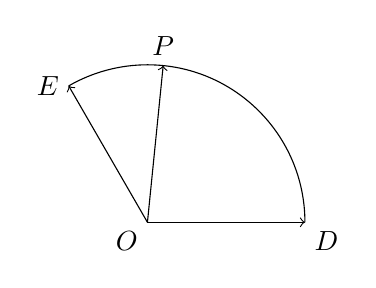
\begin{tikzpicture}[scale = 2]
						\draw[black, ->] (0, 0)--(1, 0) node at (0, 0) [anchor = north east] {\(O\)} node at (1, 0) [anchor = north west] {\(D\)};
						\draw[black, ->] (0, 0)--(0.1, {sqrt(1 - 0.01)}) node at (0.1, {sqrt(1 - 0.01)}) [anchor = south] {\(P\)};
						\draw[black, ->] (0, 0)--(-0.5, {sqrt(3) / 2}) node at (-0.5, {sqrt(3) / 2}) [anchor = east] {\(E\)};
						\draw[black] (1, 0) arc [start angle = 0, end angle = 120, radius = 1];
					\end{tikzpicture}
				\end{center}
			\end{enumerate}
			\subbigproblem
			\answord{\(t = \displaystyle \frac{1}{2}\); \(\max (x + y) = 2\).} 向量的运算, 向量的坐标表示.

			\(\ray{AC} = \ray{OC} - \ray{OA} = \displaystyle -\frac{2}{3} \vec{a} + \frac{1}{3} \vec{b}, \ray{AB} = \ray{OB} - \ray{OA} = - \vec{A} + t \vec{b}\), 于是有\(\displaystyle -\frac{2}{3} : \frac{1}{3} = -1 : t \Rightarrow t = \frac{1}{2}\).

			不妨令\(\ray{OD} = (1, 0)\)则有\(\ray{OE} = \displaystyle \left(-\frac{1}{2}, \frac{\sqrt{3}}{2}\right), \ray{OP} = (\cos \alpha, \sin \alpha)\), 其中\(\alpha \in \displaystyle \left[0, \frac{2\pi}{3}\right]\), 故
			\begin{displaymath}
				\left\{
					\begin{array}{rcl}
						x - \frac{y}{2} &=& \cos \alpha\\
						\frac{\sqrt{3}y}{2} &=& \sin \alpha
					\end{array}
				\right.
				\Rightarrow
				\left\{
					\begin{array}{rcccl}
						y &=& \frac{2\sin\alpha}{\sqrt{3}} &=& \frac{2\sqrt{3}\sin\alpha}{3}\\
						x &=& \frac{\sin\alpha}{\sqrt{3}} + \cos \alpha &=& \frac{\sqrt{3}\sin \alpha}{3} + \cos \alpha\\
					\end{array}
				\right.
			\end{displaymath}
			于是有
			\begin{displaymath}
				x+y = \sqrt{3} \sin \alpha + \cos \alpha = 2 \sin \left(\alpha + \frac{\pi}{6}\right),
			\end{displaymath}
			当且仅当\(\alpha = \displaystyle \frac{\pi}{3}\)即\(\ray{OP} = \displaystyle \left(\frac{1}{2}, \frac{\sqrt{3}}{2}\right)\), \(x+y\)取到最大值\(2\).
		\end{easonbigproblem}

	\section{附加题}
		\begin{easonbigproblem}
			已知\(\vec{a} = (3, 0), \vec{b} = (-2, 0), \abs{\vec{c}} = 1,\) 求 \(\min \ang{\vec{a} - \vec{c}, \vec{b} - \vec{c}}\).
			\subbigproblem
			\answord{\(\arccos \displaystyle \frac{-2\sqrt{6}}{7} = \pi -  \arcsin \frac{5}{7}\).} 解析几何综合.

			设\(\vec{c} = (\cos \varphi, \sin \varphi)\), 则

			\begin{align}
				\left(\vec{a} - \vec{c}\right) \cdot \left(\vec{b} - \vec{c}\right) &= \vec{a} \cdot \vec{b} - \vec{a} \cdot \vec{c} - \vec{c} \cdot \vec{b} + \vec{c} \cdot \vec{c}\\
				&= (3, 0) \cdot (-2, 0) - (3, 0) \cdot (\cos \varphi, \sin \varphi) - (\cos \varphi, \sin \varphi) \cdot (-2, 0) + (\cos \varphi, \sin \varphi)^2\\
				&= -6 - 3 \cos \varphi + 2 \cos \varphi + 1\\
				&= -\cos \varphi - 5.
			\end{align}

			又有

			\begin{align}
				\cos \ang{\vec{a} - \vec{c}, \vec{b} - \vec{c}} &= \frac{\left(\vec{a} - \vec{c}\right) \cdot \left(\vec{b} - \vec{c}\right)}{\abs{\vec{a} - \vec{c}} \cdot \abs{\vec{b} - \vec{c}}}\\
				&= \frac{- \cos \varphi - 5}{\abs{(3, 0) - (\cos \varphi, \sin \varphi)} \cdot \abs{(-2, 0) - (\cos \varphi, \sin \varphi)}}\\
				&= \frac{- \cos \varphi - 5}{\abs{(3 - \cos \varphi, - \sin \varphi)} \cdot \abs{(-2 - \cos \varphi, - \sin \varphi)}}\\
				&= \frac{- \cos \varphi - 5}{\sqrt{(3 - \cos \varphi)^2 + (- \sin \varphi)^2} \cdot \sqrt{(-2 - \cos \varphi)^2 + (- \sin \varphi)^2}}\\
				&= \frac{- \cos \varphi - 5}{\sqrt{10 - 6 \cos \varphi} \cdot \sqrt{5 + 4 \cos \varphi}}\\
				&= \frac{- \cos \varphi - 5}{\sqrt{50 + 10 \cos \varphi - 24 \cos^2 \varphi}}\\
				&\xlongequal{t\ddef \cos \varphi  \in [-1, 1]} - \sqrt{\frac{(t + 5)^2}{-24 t^2 + 10t + 50}}\\
				&\xlongequal{p\ddef t+5 \in [5, 6]} - \sqrt{\frac{p^2}{- 24p^2 + 250p - 600}}\\
				&= -\sqrt{\frac{1}{-\frac{600}{p^2} + \frac{250}{p} - 24}}\\
				&= -\sqrt{\frac{1}{-600 \left(\frac{1}{p} - \frac{5}{24}\right)^2 + \frac{49}{24}}}\\
				&\xlongequal{s=\frac{1}{p} \in \left[\frac{1}{6}, \frac{1}{4}\right]} - \sqrt{\frac{1}{-600 \left(s - \frac{5}{24}\right)^2 + \frac{49}{24}}}\\
				&\xlongequal{f=-600 \left(s - \frac{5}{24}\right)^2 + \frac{49}{24} \in \left[1, \frac{49}{24}\right]} -\sqrt{\frac{1}{f}}\\
				&\in \left[-1, -\frac{2\sqrt{6}}{7}\right],
			\end{align}

			于是有

			\begin{displaymath}
				\ang{\vec{a} - \vec{c}, \vec{b} - \vec{c}} \in \left[\arccos \left(-\frac{2\sqrt{6}}{7}\right), \pi\right].
			\end{displaymath}

			\begin{center}
				\begin{tikzpicture}
					\draw[black, ->] (-3, 0)--(4, 0) node[below] {\(x\)};
					\draw[black, ->] (0, -2)--(0, 2) node[right] {\(y\)};
 					\draw[black, very thick, ->] (0, 0)--(-2, 0) node[below] {\(\vec{b}\)};
					\draw[black, very thick, ->] (0, 0)--(3, 0) node[below] {\(\vec{a}\)};
					\draw[black] (0, 0) circle [radius = 1];
					\draw[black, fill = black] (0, 0) circle [radius = 0.05] node at (0, 0) [anchor = south east] {\(O\)};
					\draw[black, dashed] (0.5, -2)--(0.5, 2);
				\end{tikzpicture}
			\end{center}

			\calword{另解.} 设\(O(0, 0), A(3, 0), B(-2, 0), C(\cos \varphi, \sin \varphi)\). 我们首先考虑\(C \in x\)的情况, 此时夹角为\(\pi\), 显然并非最小值. 因此, \(\displaystyle P\left(\frac{1}{2}, \frac{1}{2}t\right)\)为\(\triangle ABC\)外接圆圆心, \(\odot P\)为\(\triangle ABC\)外接圆.

			若\(\odot P\)与单位圆\(\odot O\) (点\(C\)的轨迹) 相交于两点\(C, D\) (下图), 则对于\(\odot O\)的\(\arc{CD}\)上的任何一点\(G\), 都会有

			\begin{center}
				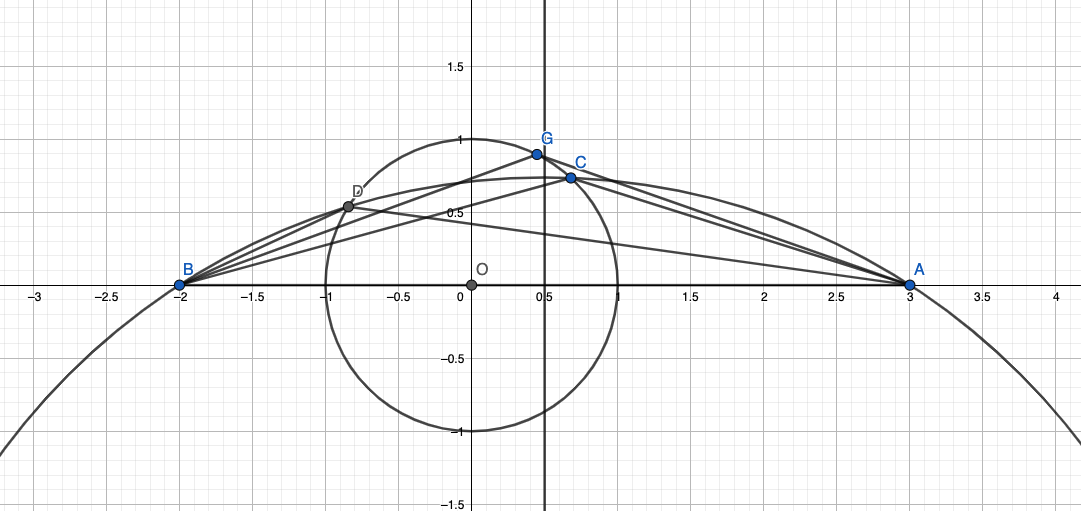
\includegraphics[scale = 0.4]{arc}
			\end{center}

			\begin{displaymath}
				\angle BCA = \angle BDA > \angle BGA,
			\end{displaymath}

			因此当\(\angle BCA\)取到最小值的时候, \(\odot P\)必然与\(\odot O\)相切, 于是有

			% \begin{displaymath}
			% 	\cos \varphi : \sin \varphi = \frac{1}{2} : \frac{1}{2} t = 1 : t \Rightarrow \sin \varphi = t \cos \varphi,
			% \end{displaymath}

			% 又有

			\begin{displaymath}
				\abs{OP} = \frac{1}{2} \sqrt{1 + t^2} = \abs{CP} - 1 = \abs{AP} - 1 = \frac{1}{2} \sqrt{25 + t^2} - 1
			\end{displaymath}

			显然有

			\begin{displaymath}
				\sqrt{1 + t^2} + 2 = \sqrt{25 + t^2},
			\end{displaymath}

			有\(t = - 2\sqrt{6}\), 外接圆半径即为\(R = \displaystyle \frac{7}{2}\).

			由正弦定理

			\begin{displaymath}
				\frac{AB}{\sin \angle BCA} = \frac{5}{\sin \angle BCA} = 2R = 7,
			\end{displaymath}

			有\(\sin \angle BCA = \displaystyle \frac{5}{7}\), 即\(\angle BCA = \displaystyle \pi -  \arcsin \frac{5}{7}\).

		\end{easonbigproblem}

	\newpage
	\bibliography{ref}
	\bibliographystyle{plain}
\end{document}